\documentclass{article}

\usepackage{tabularx}

\usepackage{graphicx}
\graphicspath{ {img/} }


\title{RAID Configuration: Pragmatic Selection Strategies}
\author{Marcel Schubert}
\date{30.03.2024}

\begin{document}
\maketitle

\section*{Introduction}
Choosing the right configuration for the logical disks
of your systems is no trivial task. But it is still one, many technicians are faced with. 
\\ \\
The goal of this report is to present pragmatic aproaches on
how to choose the right configuration for the specific task at hand. 
It does not include explanations on the underlying technical details.
It also does only apply a narrow view, and does not consider 
other factors like access protocols or optimized implementations.
But still the information can be used to calculate and compare theoretical values
to achieve more informed decisions or to do further research.
\\ \\
The methology used is simply the analysis of available information online.
Since this is not very scientific, most information was
not checked beyond plain plausibility. Also note that i did not 
make any quantifiable empirical measurements.
\\ \\
The report is divided into 5 main parts.
In the first 4, relevant information is shown
on how to compare reliability, capacity, cost and performance.
In the last section guide, a simple overarching method is presented
and this chapter also container further vendor specific information.
lastly 


\pagebreak
\tableofcontents
\pagebreak

\section{Reliability}
Since reallife situation depend on many
variables simple numeric methods are not really conlusive.
But consider the average failure time of one drive and then replicate it among
a storage group, the probability of a drive failing will obviously increase drastically
with higher numbers of drives. Analitically this change is hard to define,
since it depents on many factors. For example: it is very common,
that drives coming from the same batch of production might fail togheter
in short succession, factors like these are hard to determine. \cite{cmu:raidhighperf}


Still, if one wants to get a simple overview further i
will include formulas for the failure calculation for RAID-5
and RAID-6.
\begin{equation}
    \label{eq:r5-mttf}
    \frac{MTTF^2(disk)}{N*(G-1)*MTTR(disk)}
\end{equation}
Equation \ref{eq:r5-mttf} gives a way to calculate the mean time to failure
of RAID-5 arrays.
Where \(MTTF(disk)\) is the mean time of failure of a single disk
\(N\) is the number of disks and \(G\) is the size of the arrays.
The equation assumes no correlated failures, that means that
this simple model assume all disks are independent.
The same calculation looks slightly different for RAID-6 as seen
in eqation \ref{eq:r6-mttf}. \cite{cmu:raidhighperf}
\begin{equation}
    \label{eq:r6-mttf}
    \frac
    {MTTF^3(disk)}
    {N*(G-1)*(G-2)*MTTR^2(disk)}
\end{equation}
A overview of the amount of hardware that can fail without disrupting service can be seen in table \ref{tab:reliability}.
Notice, that in RAID-1 it also very much depends on luck where the failure happens, since if the stripes are 
favourably replicated multiple drives might be able to fail. \cite{uw:raid} 

\begin{table}[h]
    \begin{tabularx}{\textwidth}{l|X|X|X|X|X|X}
        \textbf{Level} &
        Failures \\
        \hline
        0 & 0 \\
        1 & 1 or \( \frac{n}{2} \) \\
        2 & 1 \\
        3 & 1 \\
        4 & 1 \\
        5 & 1 \\
        6 & 2 \\
       \end{tabularx}
    \caption{Amount of drives able to fail without array service degradation \cite{uw:raid}}
    \label{tab:reliability}
\end{table}
\pagebreak
\section{Capacity}
A comparative capacity calculation can relatively easily be done using table \ref{tab:capacity}.
\begin{table}[h]
    \begin{tabularx}{\textwidth}{l|X|X|X|X|X|X}
        \textbf{Level} &
        Space Efficiency \\
        \hline
        0 & n \\
        1 & \( \frac{n}{2}\)\\
        2 & \( (1-\frac{1}{n}*log_2(n+1))*full_caption \) \\
        3 & n-1 \\
        4 & n-1 \\
        5 & n-1 \\
        6 & n-2 \\
       \end{tabularx}
    \caption{Coefficient of the space multiplication (smallest disk). \cite{uw:raid} The calculation of RAID-2 was
    derived from Chen et al., Alagappan and wikipedia. \cite{cmu:raidhighperf}\cite{uw:raid}}
    \label{tab:capacity}
\end{table}
\pagebreak

\section{Cost}
An economic comparison can be created using the matrix shown in table \ref{tab:economics}.
It is feasable to compare the cost point relative to RAID level-0, since it
is the configuration with the lowest cost/efficiency rating.
To compare the different options use \( N = \textnormal{ Number of disks}\)
and with \(\max\left(x,y\right)\) is the known max function with \( x, y \in R \).
Small here refers to I/O requests of one striping unit, large refers to I/O requests of one full stripe (one stripe unit from each disk in an error-
correction group). A general overview can be seen in figure \ref{fig:costthroughput} which 
plots this againts arrays of different sizes. \cite{cmu:raidhighperf}
\begin{table}[h]
    \begin{tabularx}{\textwidth}{l|X|X|X|X|X}
        \textbf{Level} &
        Small Read &
        Small Write &
        Large Read &
        Large Write &
        Storage Efficiency \\
        \hline
        0 & 1 & 1 & 1 & 1 & 1 \\
        1 & 1 & \( \frac{1}{2} \) & 1 & \( \frac{1}{2} \) & \( \frac{1}{2} \) \\
        3 & \( \frac{1}{N} \) & \( \frac{1}{N} \) & \( \frac{N-1}{N} \) & \( \frac{N-1}{N} \) & \( \frac{N-1}{N} \) \\
        5 & 1 & \( \max\left(\frac{1}{N},\frac{1}{4}\right) \) & 1 & \( \frac{N-1}{N} \) & \( \frac{N-1}{N} \) \\
        6 & 1 & \( \max\left(\frac{1}{N},\frac{1}{6}\right) \) & 1 & \( \frac{N-2}{N} \) & \( \frac{N-2}{N} \) \\
    \end{tabularx}
    \caption{Cost Throughput Comparison relative to RAID-0 \cite{cmu:raidhighperf}}
    \label{tab:economics}
\end{table}
\pagebreak
\begin{figure}[h]
    \label{fig:costthroughput}
    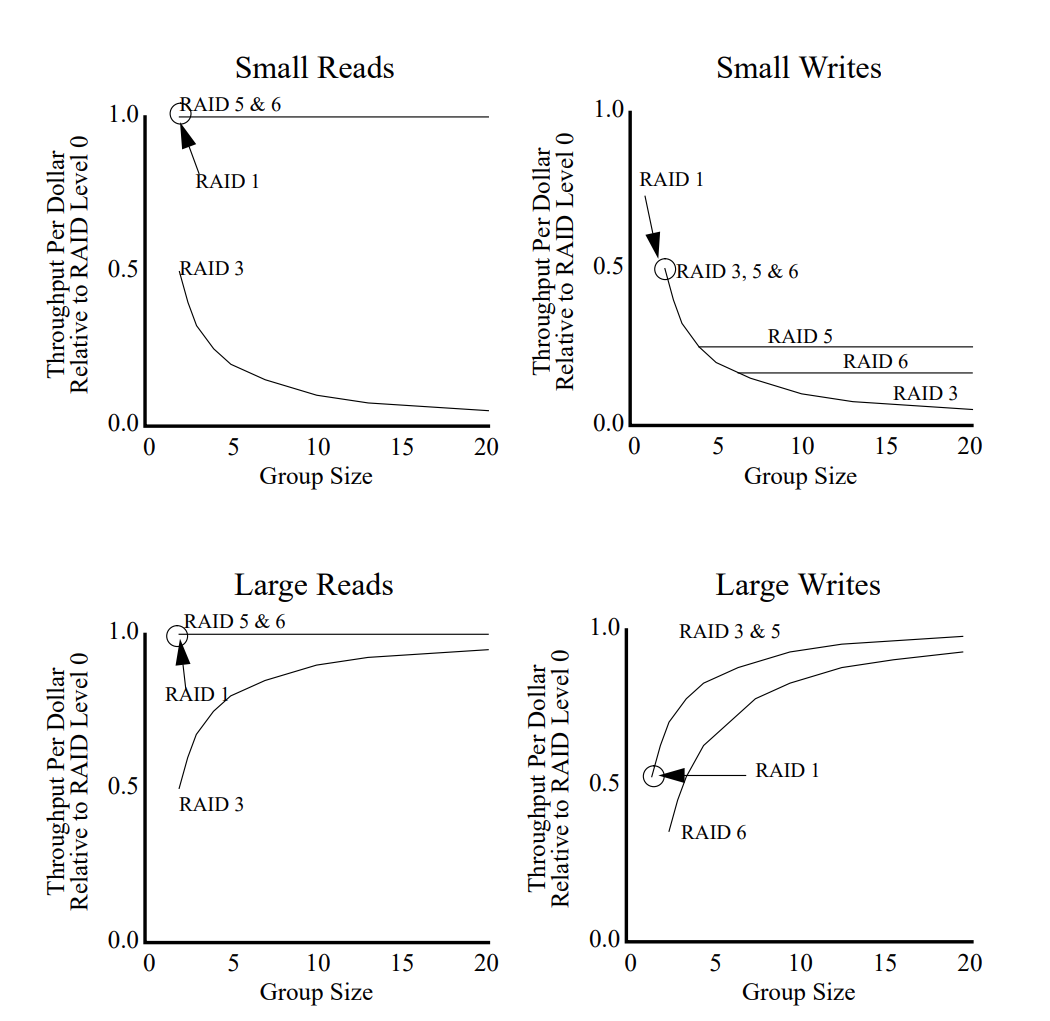
\includegraphics[width=\textwidth]{cost-troughput-comparison}
    \caption{Cost Throughput Comparison}
\end{figure}
\pagebreak
\section{Performance}
You can approximate theoretical upper bound of the performance by using table \ref{tab:perf}.
The calculation only take conceptual first order factors into account.
But despite this, it may still be benefitial to compare these fundamental boundaries
to get a general overview. The table offers the coefficients which
can be multiplied with the given drive metrics (random read, random write, seq read, seq write).
Notice, that this does not use specific block sizes, it can be applied on
average or median values. \cite{uw:raid}
\subsection{Nested RAID Configuraitions}
For nested RAID configuration, calculate the values of a single group first and
then iterate the calculation. Evenly distrubute the group size across
the total amount of disks.
For example: calculate the table then take
the values of the RAID-5 configuration an plug it into the table again.
Consider that this does not include many optimizations typically implemented
on plattforms.
Again keep in mind, that this is a rough approximation.
\begin{table}[h]
    \begin{tabularx}{\textwidth}{l|X|X|X|X|X|X}
        \textbf{Level} &
        sread &
        swrite &
        rread &
        rwrite &
        rlatency &
        wlatency \\
        \hline
        0 & n & n & n & n & 1 & 1\\
        1 & \( \frac{n}{2}\) & \( \frac{n}{2}\) & n & \( \frac{n}{2}\) & 1 & 1\\ 
        4 & n-1 & n-1 & n-1 & \( \frac{1}{2}\) & 1 & 2 \\ 
        5 & n-1 & n-1 & n & \( \frac{n}{4}\) & 1 & 2 \\
        6 & n-2 \cite{cmu:raidhighperf}& n-2 \cite{cmu:raidhighperf}& n \cite{cmu:raidhighperf}& \( \frac{n}{6} \) \cite{cmu:raidhighperf}& 1 \cite{cmu:raidhighperf}& 2 \cite{cmu:raidhighperf}\\
       \end{tabularx}
    \caption{Performance Calculation \cite{uw:raid}, The original talbe does not include RAID-6 so it was derived from Chen et al \cite{cmu:raidhighperf}}
    \label{tab:perf}
\end{table}

Notice, that with increasing number of disks
the upper bound of the throughput can be enhanced,
but generaly latency is not improved.
\subsection{Other Factors}
Always read the specific hardware as well as software manuals and documents since
theoratical speeds very much depend on the specific implementations.
Factors like controller, algorithm and cache optimization play a important role.
In the most general case, we just assume that they scale with a constant value.
\pagebreak
\section{Guide}
For a fast comparison use the Microsoft Excel workbook "raid-workbook.xlsx"
supplied with this report. Plug in the dependable variables like drive size
and io speeds and further analyze the results.
\subsection{HPE Smart Array}
HP offers different storage solutions, one of
these consists of the Smart Array Controllers,
which offer different functionalities separated by classes.
In this chapter i want to give the reader an overview and present,
what HP writes about the topics reliability, performance and efficiency.
\\ \\
There are three main classes: S,E and P.
S-Class provides a typical software RAID for MS Windows
environments and is an entry level product.
Next in line is the E-Class physical controllers
which offer enterprise level functionalities but
not all high performace optimiziations like caching.
Last in line are P-Class physical controllers
which offer typical performance oriented functionalities and optimizations
like chaching and different types of interfaces.
For the exact feature matrix consult the documentation found online. \cite{hpe:sa-userguide}
\\ \\
Performance whise HP suggests to consider, 
that the performance decreases as fault tolerance improves due to extra I/O as well as that
read performance is generally the same for all RAID levels except for smaller RAID 5 or 6 arrays. \cite{hpe:sa-userguide}
\\ \\
In their documentations they almost show the same
theoretical numbers to create a performance comparison.
They simplify their model on the basis of needed write io operations.
\begin{itemize}
    \item RAID-0, 1
    \item RAID-1/10, 2
    \item RAID-1/10 Triple, 3
    \item RAID-5, 4
    \item RAID-6, 6
\end{itemize}
This has evidently a big enough similiarity to the model used in chapter "Performance".
\\ \\
For the capacity aspects, they suggest to consider, that usable capacity decreases as 
fault tolerance improves due to an increase in parity data.
Further they say, that the usable capacity for RAID 10 and RAID 10 Triple remains flat with larger arrays and
that the usable capacity for RAID 5, 50, 6, and 60 increases with larger arrays. \cite{hpe:sa-userguide}
\\ \\
\begin{figure}
    \label{fig:hp-storage-efficiency}
    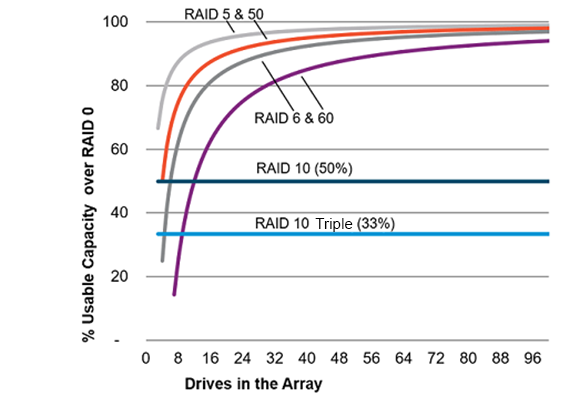
\includegraphics[width=\textwidth]{hp-storage-efficiency}
    \caption{HP Storage Efficiency \cite{hpe:sa-userguide}}
\end{figure}
Figure \ref{fig:hp-storage-efficiency} shows a general plot of the storage efficiency development
over a increasing amount of disks. The plot assumes the group size 2 for RAID-50 and RAID-60. \cite{hpe:sa-userguide}
\\ \\
At last consider following suggestions by HP:
\begin{itemize}
    \item RAID 1/10 Triple: Optimize for fault tolerance and write performance.
    \item RAID 6/60: Optimize for fault tolerance and usable capacity.
    \item RAID 1/10: Optimize for write performance.
    \item RAID 5/50: Optimize for usable capacity.
\end{itemize}

\section*{Fun Facts}
It appears to be, that RAID was an abreviation for "Redundant Array of Inexpensive Disks" befoire beeing
modified to the more known version of: "Redundant Array of Independent Disks"
Source is: trust me brother, cannot be bothered to look it up.
\listoffigures
\listoftables
\bibliographystyle{ieeetr}
\bibliography{refs}
\begin{figure}[h]
    \label{fig:raid-overview}
    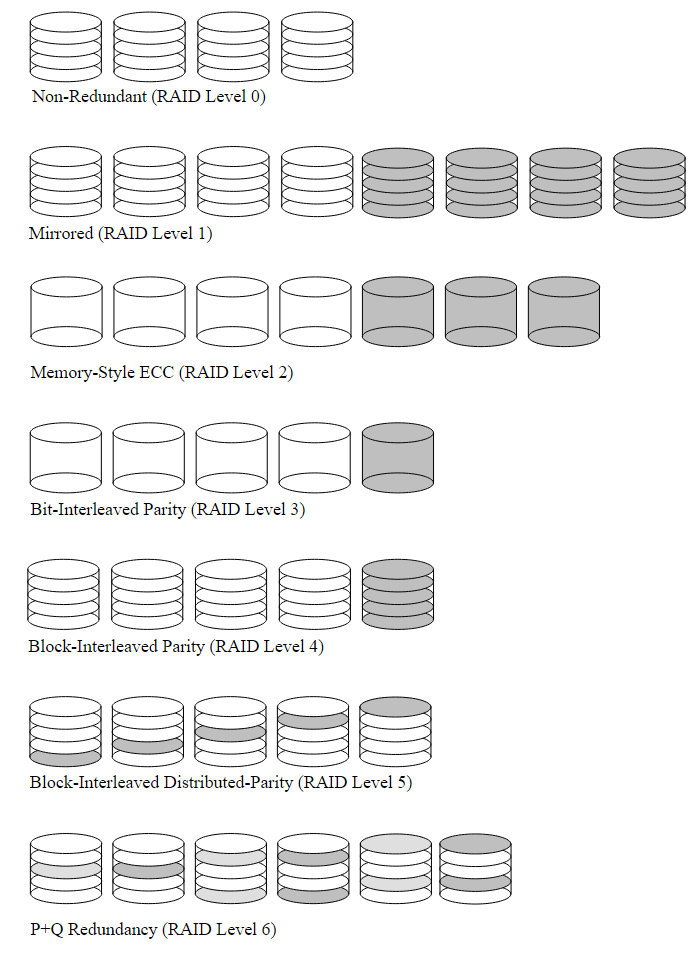
\includegraphics[width=\textwidth]{raid-overview}
    \caption{Raid Overview \cite{cmu:raidhighperf}}
\end{figure}
\end{document}